\Section{Транспортные механизмы архитектуры TCP/IP}{Лекции 3-4}{Игорь Смирнов}

\begin{itemize}
    \item Дейтаграммный обмен
    \begin{itemize}
        \item Не гарантирует последовательность доставки
        \item Не обеспечивает квитирование (нет сообщения о том, что пакет успешно доставлен)
        \item В TCP/IP реализуется протоколом UDP
    \end{itemize}
    \item Потоковый обмен
    \begin{itemize}
        \item Создаётся виртуальный канал (поток)
        \item Последовательность доставки гарантируется
        \item Обеспечивается подтверждение доставки
        \item Бывает однопоточным (протокол TCP) и многопоточным (протокол SCTP)
    \end{itemize}
\end{itemize}

\Subsection{Протокол UDP}

Used Datagram Protocol

По сравнению с другими транспортными протоколами имеет более высокую скорость и менее надёжен.

Зарезервирован номер 17 в IP-пакете. 

Для адресации используются UDP-порты.

Сервер {\it обычно} использует фиксированные номера портов.

Клиент {\it обычно} использует непривилегированные номера портов (обычно случайные).

Клиент должен знать, по какому порту стучаться на сервер, а сервер просто отвечает на тот же порт.

Весь обмен определяется двумя IP-адресами и двумя номерами портов.

\Subsubsection{Формат пакета UDP}

\begin{figure}[H]
  \centering
  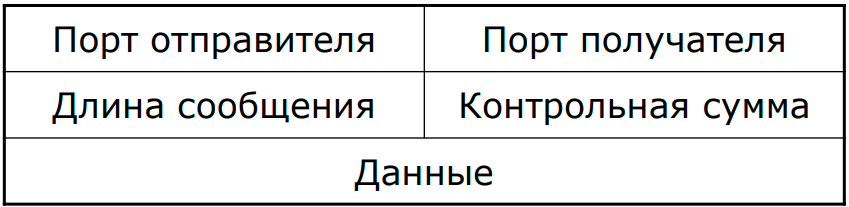
\includegraphics[width=15cm]{images/03/01}
\end{figure}

Длина сообщения~--- длина UDP дейтаграммы.

Контрольная сумма считается по всему пакету (а в IP только по заголовку).

Если контрольная сумма равна 0, то она не вычислялась (например, если мы верим, что у нас сверхнадёжный канал).

Контрольная сумма вычисляется с учётом псевдозаголовка.

\begin{figure}[H]
  \centering
  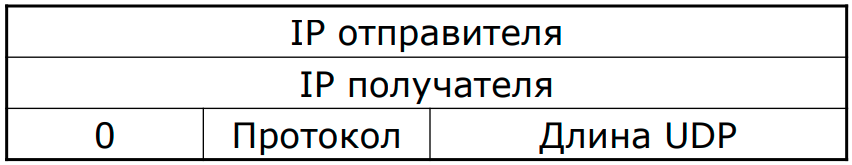
\includegraphics[width=15cm]{images/03/02}
\end{figure}

Благодаря этому, если у нас была произведена атака и были подменены IP-адреса, а контрольную сумму злоумышленник не пересчитал, то она не сойдётся (скорее всего).

Поэтому злоумышленнику нужно сохранить к себе весь пакет и пересчитать контрольную сумму (ага, очень большая проблема для него).

Приложения, использующие UDP:
\begin{itemize}
    \item TFTP (69)
    \item DNS (53)
    \item SNMP (161, 162)~--- протокол управляющих сообщений
    \item BOOTP, DHCP (67, 68)~--- получение параметров IP
    \item RIP (520)~--- маршрутизация
\end{itemize}

\Subsection{Протокол TCP}

Transmission Control Protocol

По сравнению с UDP имеет:
\begin{itemize}
    \item Более низкую скорость
    \item Большую надёжность
\end{itemize}

Зарезервирован номер 6 в IP-пакете.

Адресация с помощью TCP-портов.

Передача~--- потоковая. Данные для передачи хранятся в буффере. Это единственный протокол, который имеет дело не с пакетами, а с двумя очередьми: буффером приёма и передачи. В отличие от UDP, оперируем сегментами, а не пакетами. Можем захотеть передать 100 байт, но они добавятся в общую очередь и за раз передастся 1000 байт.

Данные добавляются в конец буффера, а передаются из начала. 

Каждый передаваемый байт пронумерован. Сегменту присваивается номер его первого байта (номер очереди).

При посылке в сеть сегмента, он копируется в буффер повторной передачи, заводится таймаут. Если в течение таймаута не получили подтверждение, посылаем снова. И так делается (по дефолту) до 5 раз.

Каждый переданный байт должен быть подтверждён. При получения подтверждения от сегмента, подтверждёнными считаются все байты сегмента. Подтверждение содержит номер следующего ожидаемого байта.

\begin{figure}[H]
  \centering
  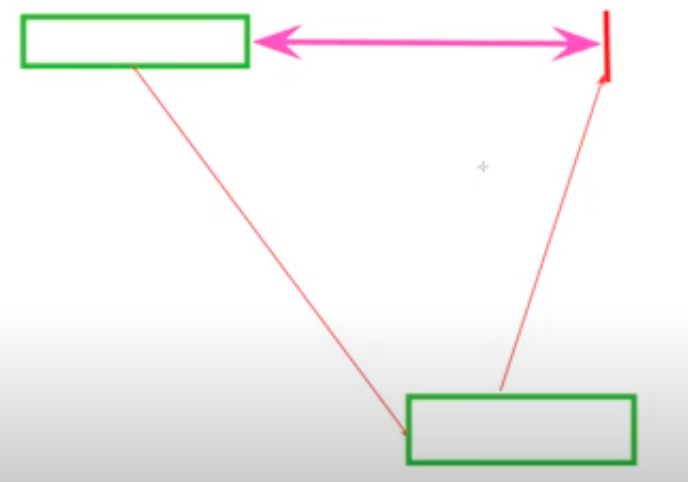
\includegraphics[width=15cm]{images/03/03}
\end{figure}

В момент времени $T_1$ Алиса послала сообщение Бобу.

В момент времени $T_2$ Боб это сообщение получил и отправил подтверждение Алисе.

В момент времени $T_3$ Алиса получила подтверждение от Боба и может отправлять второй пакет. Таким образом, мы получили простой передачи $T_3-T_1$.

В TCP отрицательные квитанции не посылаются. Например, если у нас не сошлась контрольная сумма, нам не пошлют сообщение об ошибке. Принимающая сторона просто не будет посылать подтверждение получения и мы попробуем отправить пакет снова.

\Subsubsection{Формат TCP пакета}

\begin{figure}[H]
  \centering
  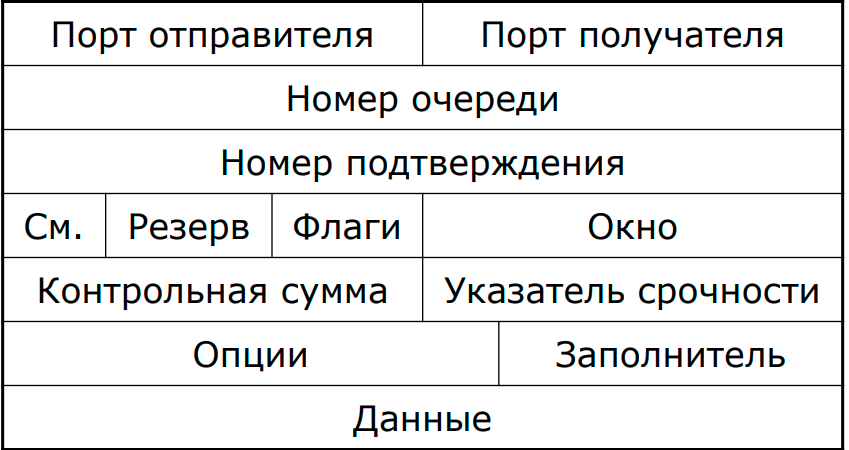
\includegraphics[width=15cm]{images/03/04}
\end{figure}

\begin{itemize}
    \item Номер очереди~--- номер посланного сегмента при обмене или синхронизация номеров сегментов при установлении соединения
    \item Номер подтверждения~--- подтверждение принятого сегмента или синхронизация номеров сегментов при установлении соединения
    \item Смещение данных~--- длина заголовка TCP (и так же, как и в IP, с помощью него понимаем, есть у нас опции или нет)
    \item Окно~--- величина скользящего окна (о нём позже)
    \item Контрольная сумма~--- по всему высылаемому сегменту
    \item Указатель срочности~--- объём срочных данных

\end{itemize}

{\bf Флаги}

\begin{figure}[H]
  \centering
  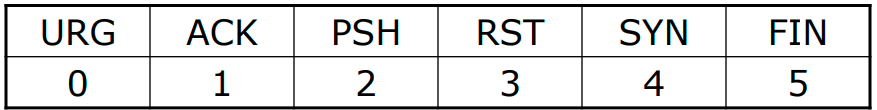
\includegraphics[width=15cm]{images/03/05}
\end{figure}

\begin{itemize}
    \item URG~--- флаг срочности. Задействовано поле <<Указатель срочности>>. Это позволяет передать определённый объём данных в сеть без буфферизации. Пример, когда надо: управление удалённым терминалом, компьютерные игры.
    \item ACK~--- флаг подтверждения. Задействовано поле <<Подтверждение>> и в этом пакете у нас находится квитанция.
    \item PSH~--- флаг проталкивания. О нём позже.
    \item RST~--- флаг сброса. Перезагрузка соединения
    \item SYN~--- флаг синхронизации. Синхронизация номеров очередей для создания виртуального канала. Первый пакет с каждой стороны должен иметь установленным этот флаг
    \item FIN~--- флаг закрытия соединения. Завершение соединения
\end{itemize}

\Subsubsection{Установка соединения}

Хотим начать соединение. Нужно договориться, с какого номера клиент и сервер будут начинать отсчёт отправляемых сообщений. Казалось бы, можно начать с нуля (сначала даже так и делали), но выяснилось, что так хакерам проще вклиниться в уже установленное TCP соединение.

Поэтому решили номер первого сегмента генерировать случайно. 

Таким образом, вся установка соединения~--- двусторонний обмен номерами сегментов между отправляющей и принимающей сторонами.

\begin{enumerate}
    \item A посылает B пакет с флагом SYN, в котором указан номер первого сегмента минус единица ($N_{seqA}$)
    \item B посылает в ответ пакет с флагом ACK и $N_{ackB}=N_{seqA}+1$
    \item B посылает A пакет с флагом SYN и $N_{seqB}$
    \item A посылает B подтверждение о синхронизации с флагом ACK и $N_{ackA}=N_{seqB}+1$
\end{enumerate}

С этого момента каждый знает номер очереди собеседника и можно проводить штатный обмен.

{\bf НО!} в пакетах, отсылаемых в сообщениях 2 и 3 нет общих полей. Поэтому решили это передавать одним пакетом.

Это называется трёхпутевой схемой организации соединения.

\Subsubsection{Разрыв соединения}

\begin{enumerate}
    \item A посылает B пакет с флагом FIN
    \item B посылает A пакет с флагом ACK 
    \item B посылает A пакет с флагом FIN
    \item A посылает B пакет с флагом ACK
\end{enumerate}

\Subsubsection{Конечный автомат протокола TCP}

Как работает TCP:

\begin{itemize}
    \item На сервере есть сокет (допустим, на порту 80).
    \item Когда приходит запрос на соединение, пораждается ещё один сокет (с тем же номером порта)~--- рабочий. И именно с ним работает клиент. А прошлый сокет остался в состоянии слушания входящих соединений.
    \item У рабочего сокета может быть несколько состояний.
    \item Стоит заметить, что ничего страшного в том, что у рабочего сокета такой же номер порта нет, так как сокет определяется ещё и IP-адресом клиента.
\end{itemize}

\begin{figure}[H]
  \centering
  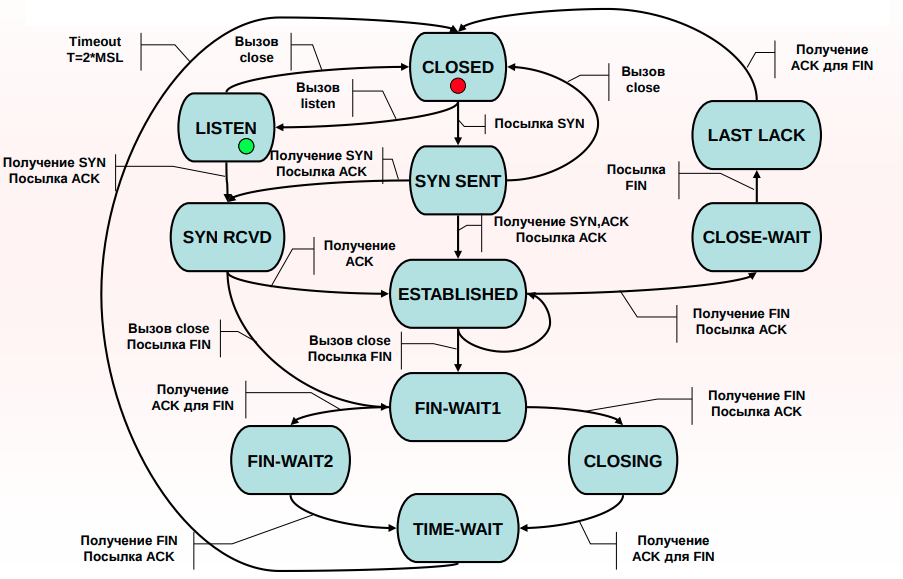
\includegraphics[width=15cm]{images/03/06}
\end{figure}

На сервере решили организовать слущающий сокет. Сделали системный вызов listen. Сокет першёл в состояние LISTEN.

Если получили сигнал SYN, у нас породился второй сокет, красный продолжает слушать, а зелёный переходит в состояние SYN RCVD.

Получили ACK и перешли в состояние ESTABLISHED. В этом состоянии происходит вся передача данных. Все остальные состояния~--- служебные.

Пусть мы вызвали {\tt close}. Тогда перейдём в состояние FIN-WAIT1, получим ACK, перейдём в FIN-WAIT2, получим FIN, отправим ACK, перейдём в TIME-WAIT. Это долгое состояние, в котором мы разгребаем весь мусор из сети. Там ждём от полутора до трёх минут, собирая все приходящие данные, после чего переходим в CLOSED.

Есть утилита {\tt netstat}, которая позволяет посмотреть на сокеты и их состояния. Там скорее всего вы увидите толко LISTEN, ESTABLISHED и TIME-WAIT. Все остальные состояния очень быстрые.

Это было для сервера. А клиент посылает SYN, переодит в SYN SENT, ну а дальше всё так же.

\Subsubsection{Срочные данные}

URG~--- немедленная доставка данных приложению на приёмной стороне.

URG~--- флаг наличия срочных данных.

Offset~--- указатель на первые несрочные данные.

Проталкивание данных~--- немедленная отсылка сегмента в сеть. 

\Subsubsection{Управление скоростью передачи}

Идея: давайте передавать не один, а несколько сегментов и будем ждать от всех них подтверждения.

В сеть могут передаваться сегменты, которые попали в {\bf скользящее окно}.

Обычно скользящее окно кратно размеру сегмента.

Сдвиг окна происходит, когда получаем подтверждение на первый посланный сегмент.

Хотим послать в сеть 4 сегмента. И скользящее окно их покрывает. Посылаем сразу 4 сегмента и ждём подтверждений. 

Пришло подтверждение на первый сегмент~--- сдвигаем окно на величину подтверждённых данных.

Если пришло подтверждение на более поздний сегмент, это запоминается, но окно не сдвигается, пока не пришло подтверждение на самый левый из неподтверждённых сегментов.

Идеальная ситуация~--- когда подтверждение на первый сегмент приходит ровно тогда, когда мы отправили последний. Если мы так подобрали размер скользящего окна, то мы достигли максимальной возможной скорости передачи по TCP.

По ходу передачи размер окна меняется. Это всё настраивается в опциях.

{\bf Куллстори.} Раньше предлагали скачать приложения, которые ускорят ваш интернет. В 99\% случаев это были троянские кони, а 1\%~--- утилита, которая оценивала скорость связи и прописывала в реестр оптимальный размер скользящего окна.

\Subsubsection{Протоколы, использующие TCP}

\begin{itemize}
    \item telnet (23)~--- удалённый терминал
    \item SMTP (25)~--- почта
    \item FTP (20, 21)~--- передача файлов
    \item DNS (53)
    \item HTTP (80)
    \item POP3 (110)
    \item IMAP4 (143)
    \item SSH (22)
    \item ...
\end{itemize}

\Subsection{Протокол SCTP}

Stream Control Transmission Protocol

Хочется:
\begin{itemize}
    \item Объединить достоинства UDP и TCP
    \item Исправить недостатки UDP и TCP
\end{itemize}

Он позволяет внутри одного соединения организовывать несколько потоков.

Пакет состоит из заголовка и нескольких субпакетов (чанков).

\begin{figure}[H]
  \centering
  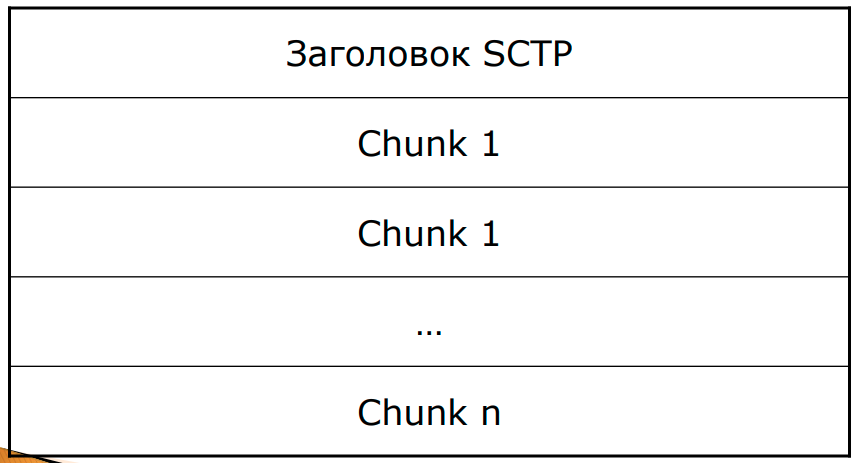
\includegraphics[width=15cm]{images/03/07}
\end{figure}

Каждый субпакет имеет свой заголовок и данные

Зачем может понадобится несколько потоков? Когда мы передаём данные разного размера, разного назначения, разной скорости.

Например, по одному передаём громадные файлы, по второму~--- сообщения, по третьему~--- управляющие команды.

По сути мы заменяем несколько TCP сокетов на один SCTP.

Формат заголовка:

\begin{figure}[H]
  \centering
  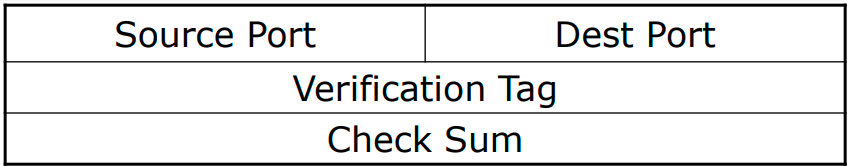
\includegraphics[width=15cm]{images/03/08}
\end{figure}

Verification Tag~--- метка для проверки отправителя пакета. Замена аутентификации.

Формат субпакета:

\begin{figure}[H]
  \centering
  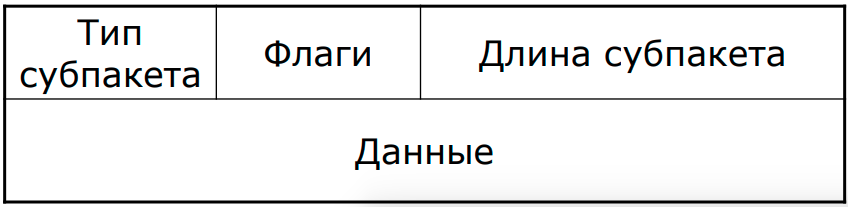
\includegraphics[width=15cm]{images/03/09}
\end{figure}

Тип субпакета~--- число от 0 до 255
\begin{itemize}
    \item 0~--- полезные данные
    \item >0~--- служебная информация
\end{itemize}

Флаги~--- служебные разряды. Определяются типом субпакета.

Особенности:
\begin{itemize}
    \item Многопоточность
    \item Мультидомность~--- SCTP может использовать сразу несколько каналов. Например. если один вышел из строя, можем использовать другой.
    \item Проверка подлинности
    \item Подтверждение приёма
    \item Средства устранения перегрузок
    \item Передача пакетами (а не как в TCP)
\end{itemize}